\cleardoublepage
\markboth{E. YOLO BALL DETECTOR TRAINING RESULTS}{}
\chapter{YOLO Ball Detector Training Results}

\begin{figure}[htbp]
\centering
\caption{\textit{YOLOv26s ball detector training curves: loss, precision, recall, and mAP over 75 training epochs.}}
\label{fig:e1}
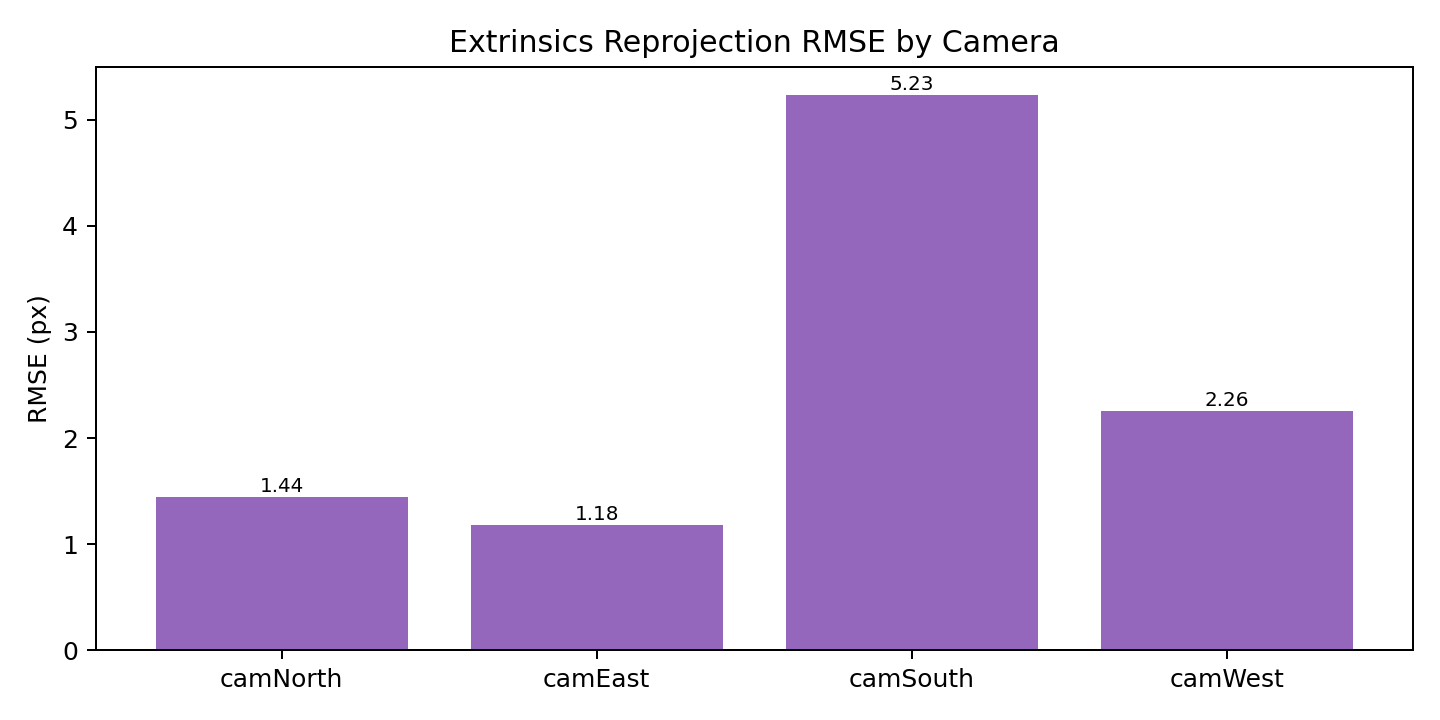
\includegraphics[width=0.9\textwidth]{figures/yolo_training_curves}
\end{figure}

\begin{figure}[htbp]
\centering
\caption{\textit{Normalised confusion matrix for the YOLOv26s ball detector on the validation set.}}
\label{fig:e2}
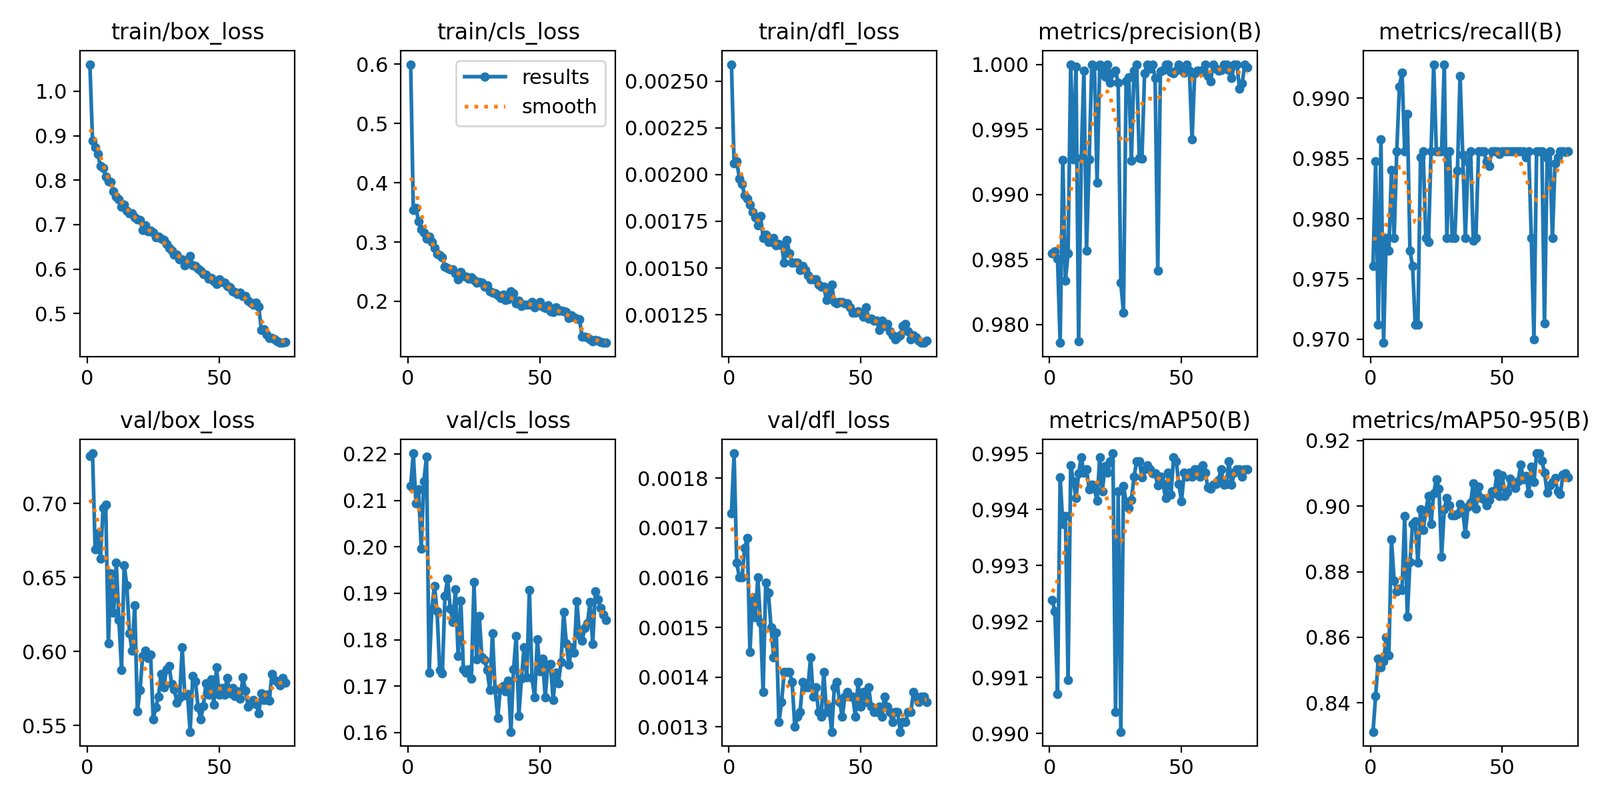
\includegraphics[width=0.75\textwidth]{figures/yolo_confusion_matrix}
\end{figure}

\begin{figure}[htbp]
\centering
\caption{\textit{Precision-Recall curve for the YOLOv26s ball detector.}}
\label{fig:e3}
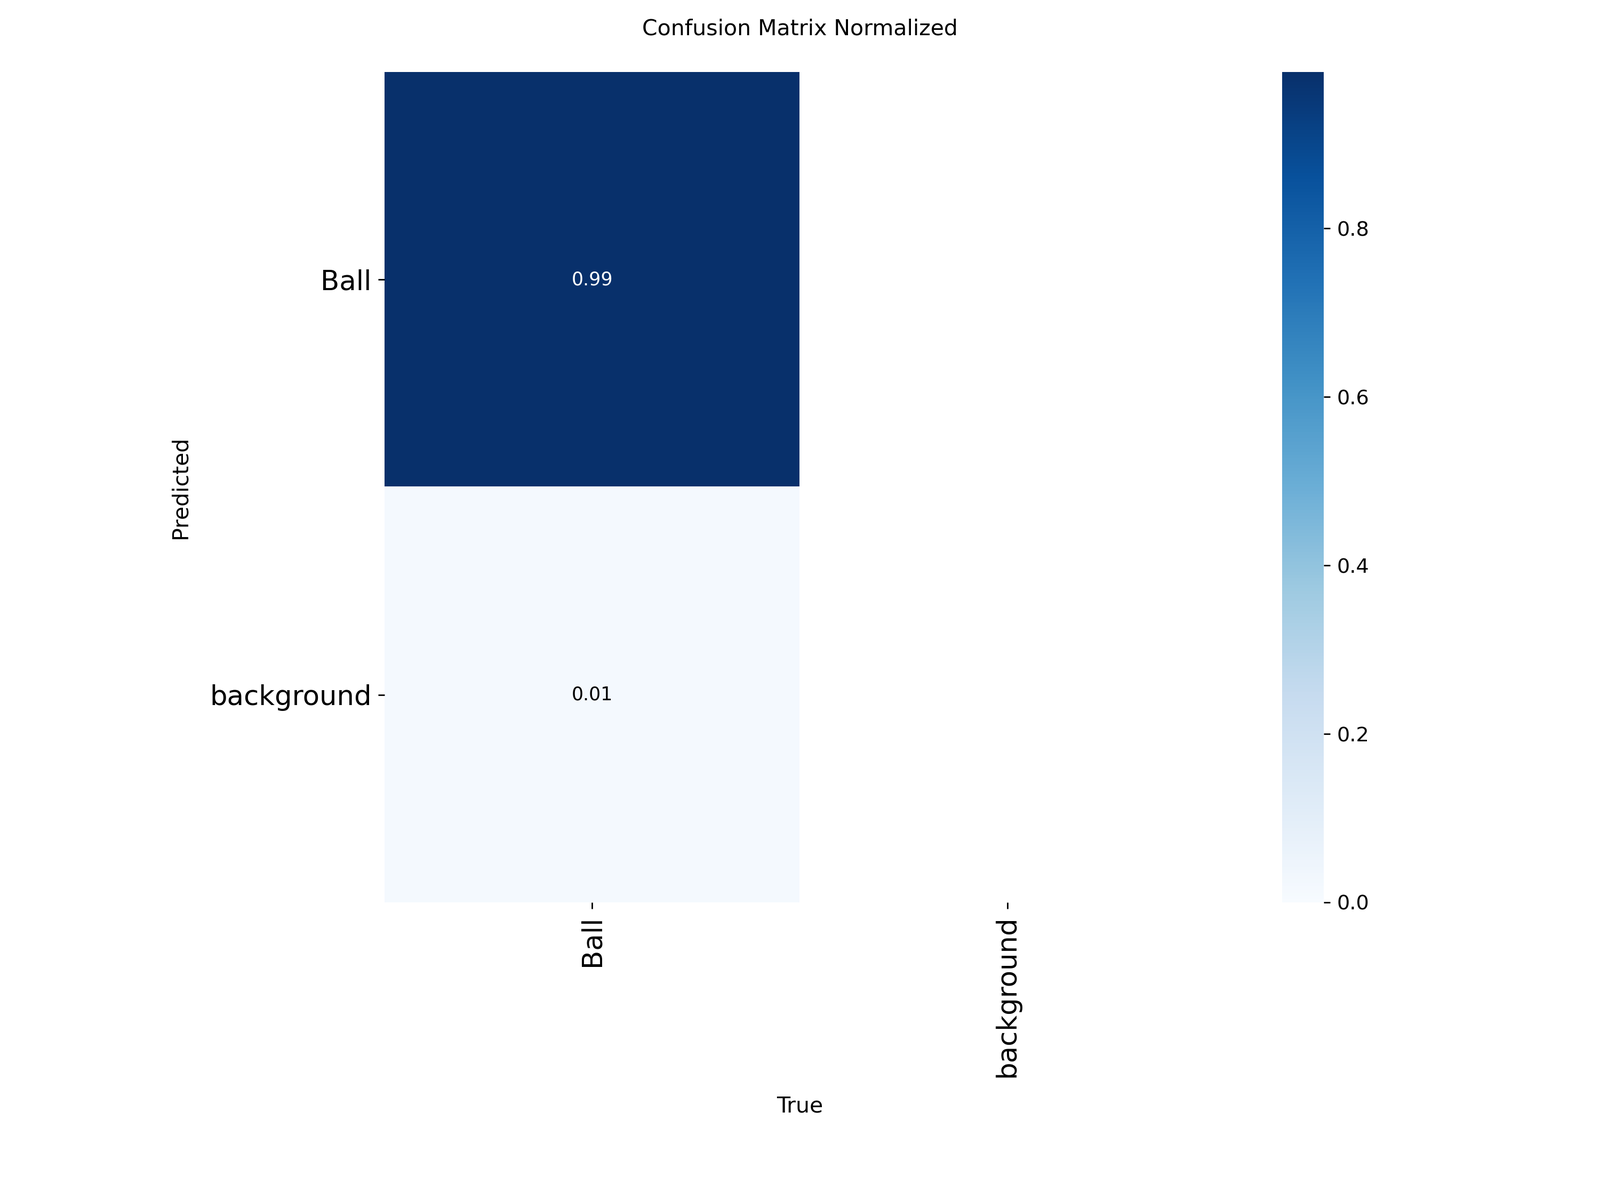
\includegraphics[width=0.75\textwidth]{figures/yolo_pr_curve}
\end{figure}

\begin{figure}[htbp]
\centering
\caption{\textit{Sample training batch: YOLOv26s ball detection annotations on training images.}}
\label{fig:e4}
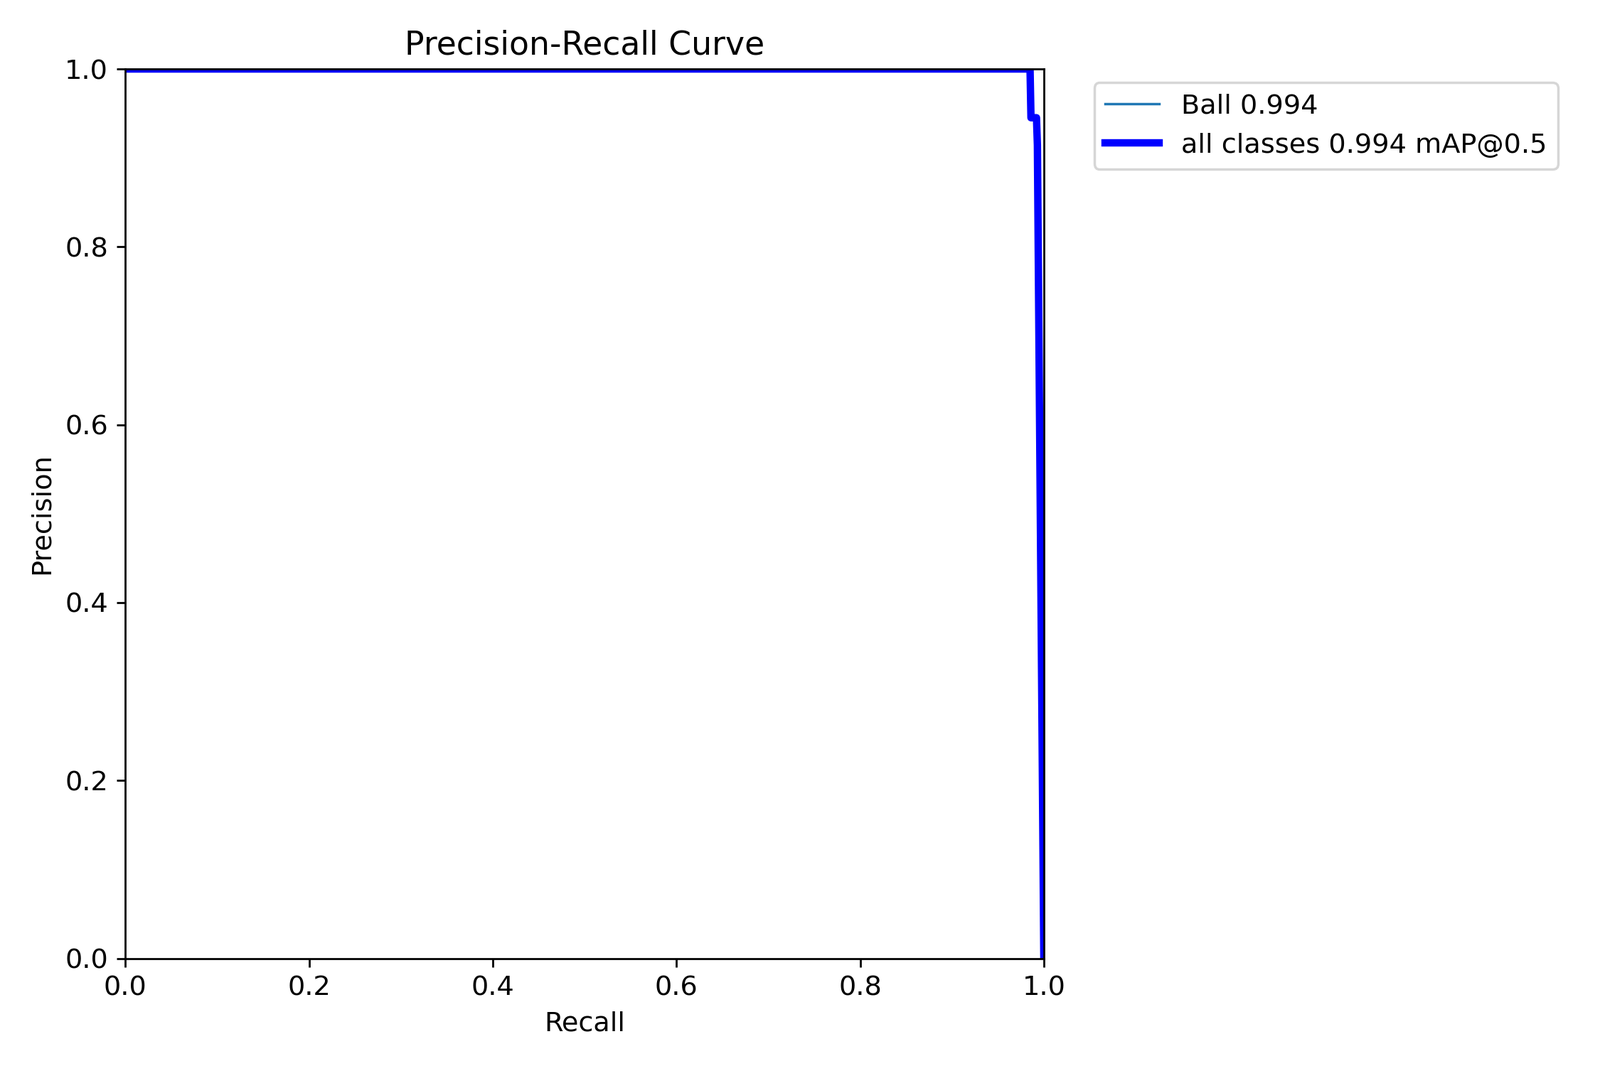
\includegraphics[width=0.9\textwidth]{figures/yolo_sample_batch}
\end{figure}

\begin{figure}[htbp]
\centering
\caption{\textit{Validation predictions vs ground truth.}}
\label{fig:e5}
\begin{subfigure}[b]{0.45\textwidth}
\centering
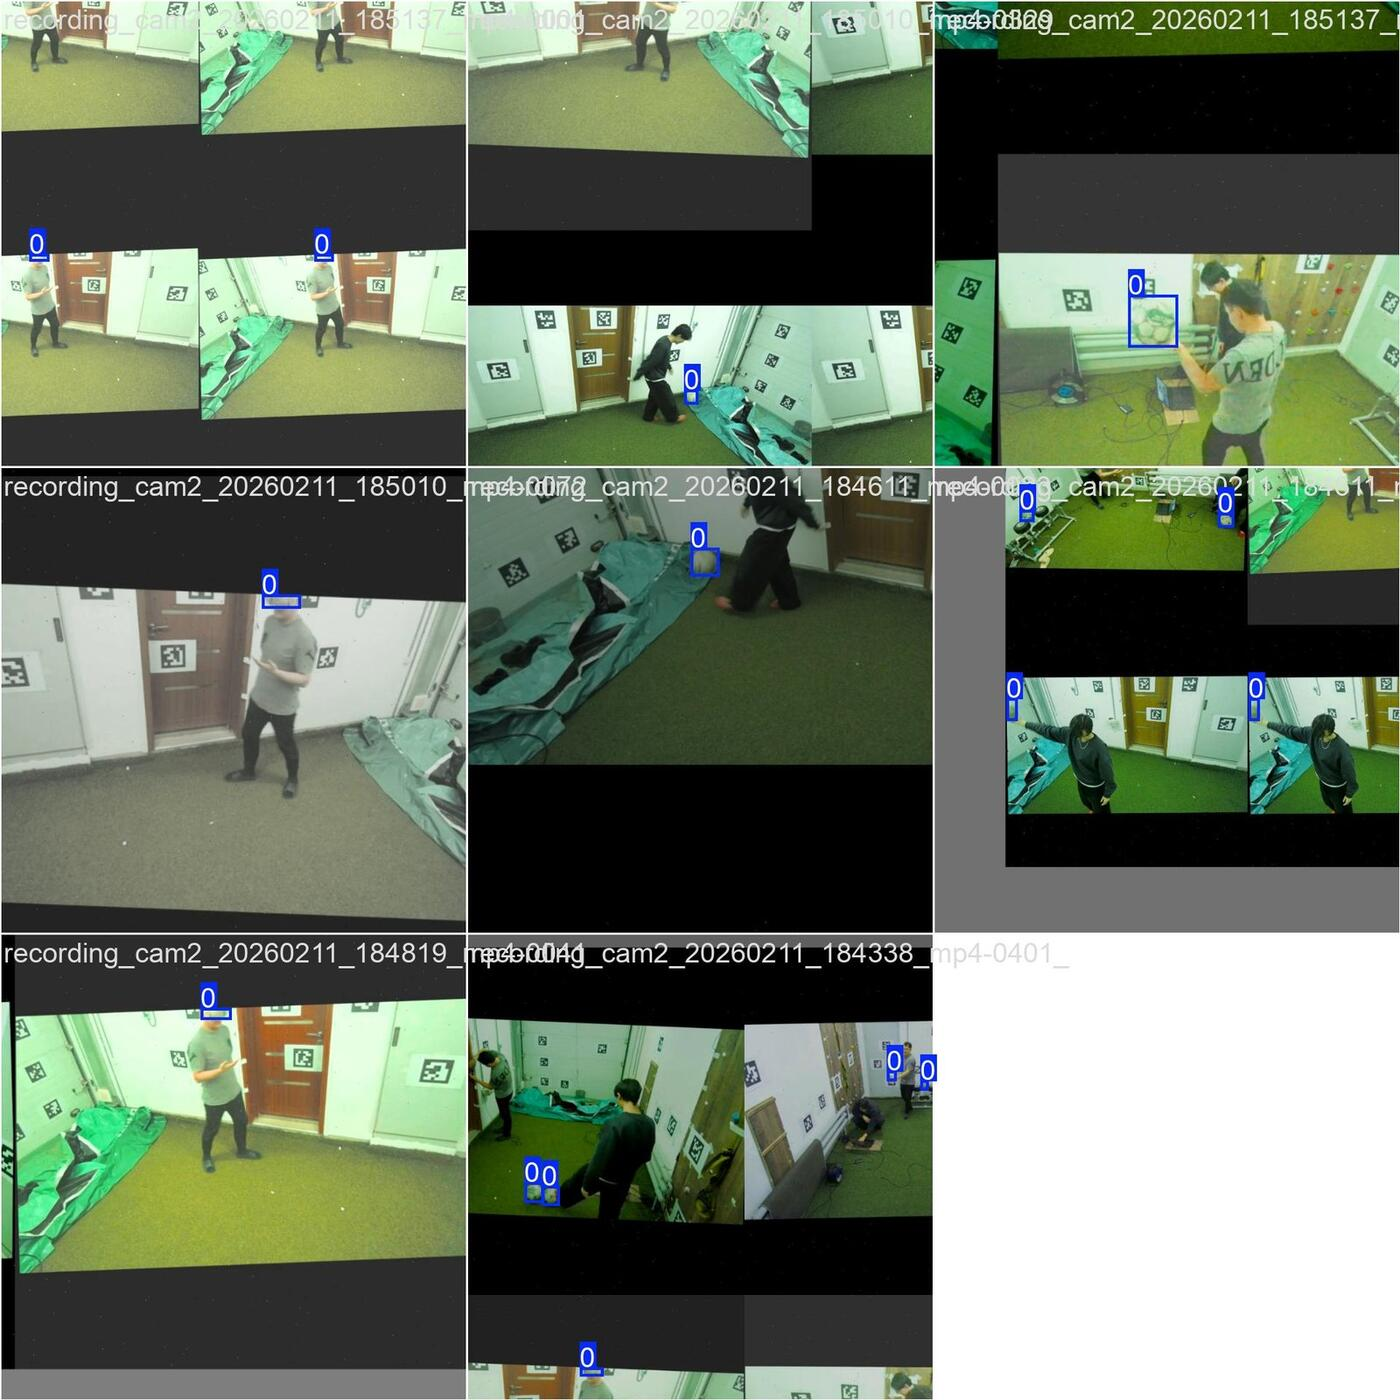
\includegraphics[width=\textwidth]{figures/yolo_val_pred_a}
\caption*{(a)}
\end{subfigure}
\hfill
\begin{subfigure}[b]{0.45\textwidth}
\centering
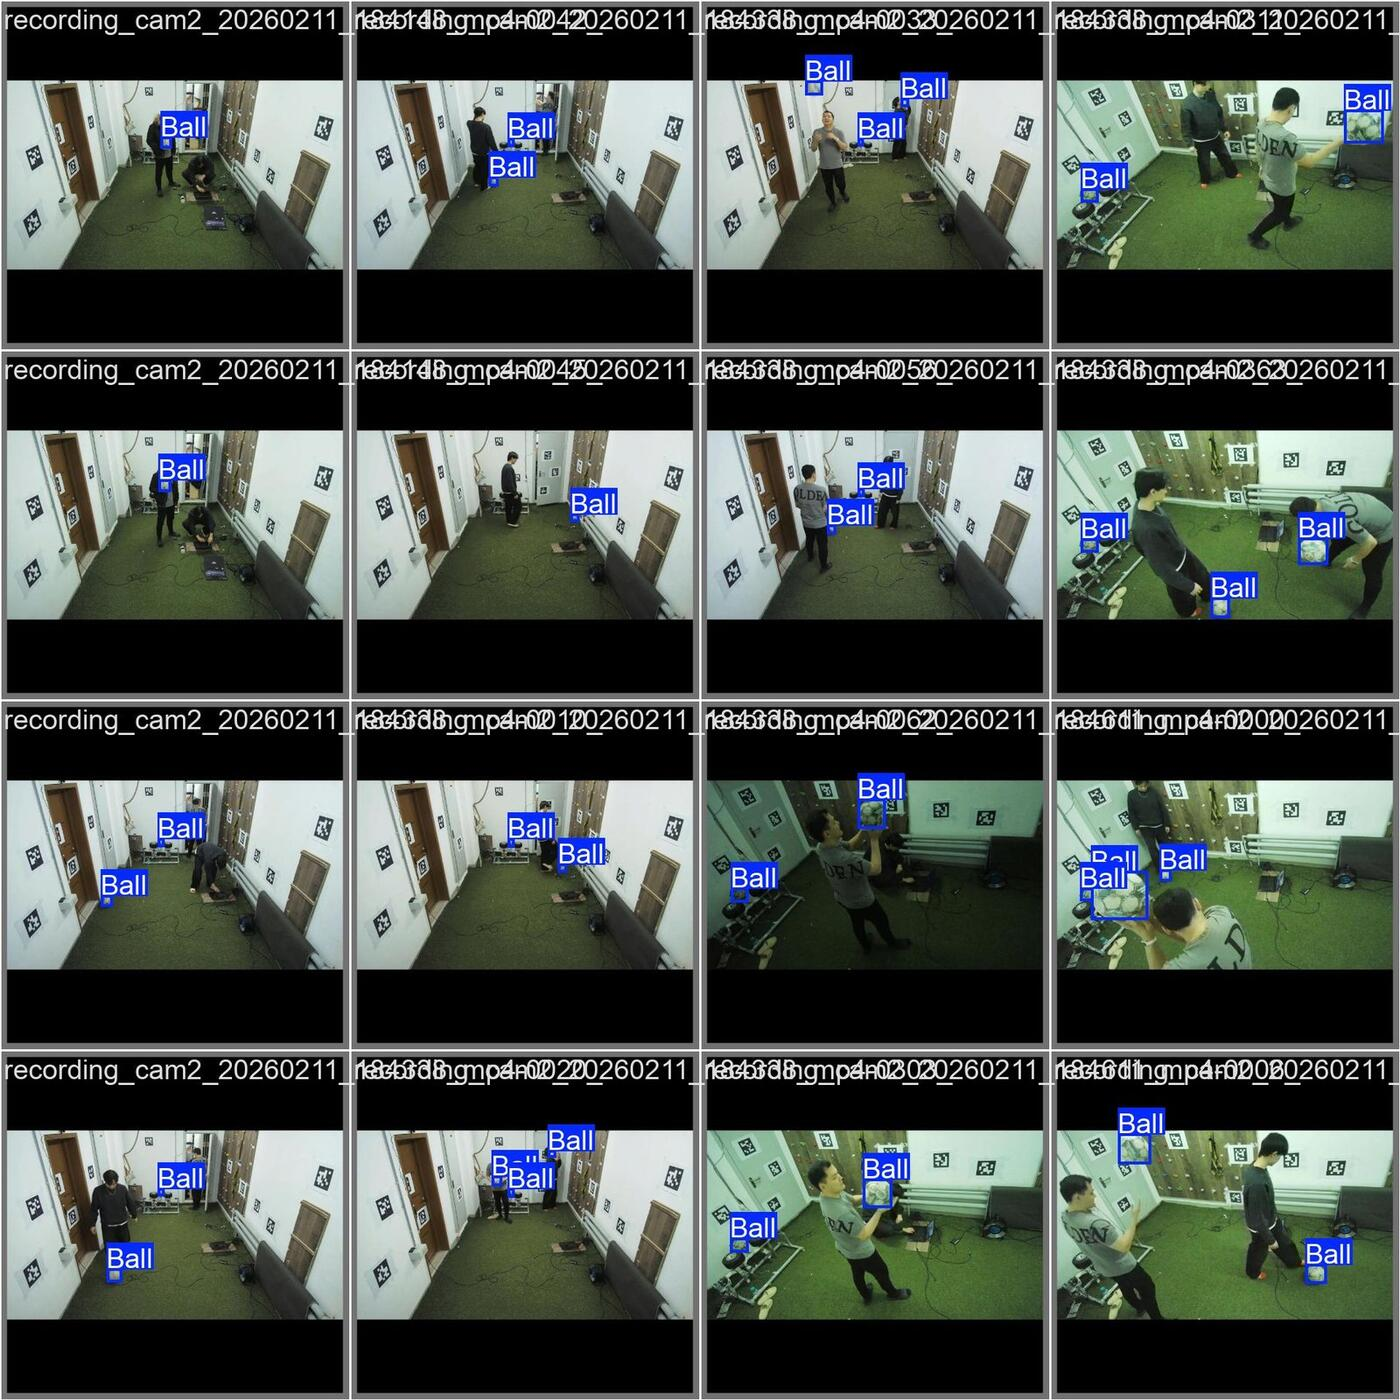
\includegraphics[width=\textwidth]{figures/yolo_val_pred_b}
\caption*{(b)}
\end{subfigure}
\end{figure}
